\documentclass[10pt,twocolumn]{article}

\usepackage[margin=0.85in]{geometry}
\usepackage{amsmath,amssymb}
\usepackage{graphicx}
\usepackage{booktabs}
\usepackage{multirow}
\usepackage{hyperref}
\usepackage{xcolor}
\usepackage{caption}
\usepackage[numbers]{natbib}

\captionsetup{font=small, labelfont=bf}

\title{AdaDion V2 on CIFAR-10: Benchmarking Adaptive Low-Rank Orthogonal Optimizers for Vision Models}

\author{
  Ansh Tiwari \\
  \texttt{ansschh@github}
}

\date{}

\begin{document}
\maketitle

\begin{abstract}
We benchmark AdaDion V2, an adaptive-rank variant of the Dion optimizer, against AdamW, Muon, Dion, and Dion2 on CIFAR-10 with ResNet-18 and ViT-Small. After identifying and correcting three implementation issues related to parameter coverage, mixed-precision interaction, and learning rate calibration, AdaDion V2 achieves 96.20\% on ResNet-18 (3 seeds), outperforming Dion (95.97\%), Muon (95.87\%), and AdamW (95.29\%). On ViT-Small, the Dion family (Dion 92.38\%, AdaDion 92.25\%, Dion2 92.24\%) outperforms Muon (88.86\%) and AdamW (83.65\%). A 22-run ablation isolates the contribution of each design choice: learning rate is the dominant factor, adaptive rank adds 0.18\% over non-adaptive Dion, and gradient clipping at 1.0 is optimal.
\end{abstract}

\section{Introduction}

Spectral optimizers apply orthogonal or low-rank projections to gradient updates, replacing the diagonal scaling of AdamW with matrix-valued preconditioning. Muon~\cite{jordan2024muon} uses Newton-Schulz iteration for orthogonalization. Dion~\cite{ahn2024dion} uses low-rank power iteration with compressed communication. Dion2 extends Dion with fraction selection and Newton-Schulz. AdaDion V2 adds adaptive rank selection to Dion, dynamically adjusting the low-rank factor based on effective rank tracking.

These optimizers were developed for large-scale LLM pretraining with distributed parallelism (FSDP, tensor parallelism). All prior evaluations used transformer models with natively 2D weight matrices. This report evaluates them on CIFAR-10 image classification, where convolutional architectures introduce 4D weight tensors and the model scale is orders of magnitude smaller.

\section{Setup}

\subsection{Models and Data}

We use ResNet-18 (11.2M parameters) and ViT-Small (10.7M parameters, patch size 4, 6 layers, 384-dim, 6 heads) on CIFAR-10. Data augmentation includes random crop with padding 4, horizontal flip, AutoAugment (CIFAR-10 policy), random erasing ($p=0.1$), and label smoothing ($\epsilon=0.1$). ViT-Small uses stochastic depth (linearly increasing to 0.1).

\subsection{Optimizers}

All spectral optimizers use a hybrid parameter grouping: 2D weight matrices use the spectral update rule, while 1D parameters (norms, biases) use AdamW. For Dion, Dion2, and AdaDion V2, 4D convolutional weights are reshaped to 2D via a flatten wrapper that converts $(C_\text{out}, C_\text{in}, k, k) \to (C_\text{out}, C_\text{in} k^2)$ before each optimizer step and restores the shape afterward. Muon handles this internally via its \texttt{flatten} parameter. Table~\ref{tab:optconfigs} lists the configurations used. All spectral optimizers run in float32 without mixed precision (Section~\ref{sec:amp}).

\begin{table}[t]
\centering
\caption{Optimizer configurations for ResNet-18.}
\label{tab:optconfigs}
\small
\begin{tabular}{@{}lll@{}}
\toprule
Optimizer & Key parameters & Scalar LR \\
\midrule
AdamW & lr=1e-3, wd=0.05, $\beta$=(0.9, 0.999) & -- \\
Muon & lr=0.02, $\mu$=0.95, nesterov, rms\_norm & 1e-3 \\
Dion & lr=0.02, rank\_frac=0.25, wd=0.01 & 1e-3 \\
Dion2 & lr=0.02, frac=0.25, ef\_decay=0.95 & 1e-3 \\
AdaDion & lr=0.01, $\mu$=0.95, wd=0.1, adaptive & 0.01 \\
\bottomrule
\end{tabular}
\end{table}

\subsection{Training}

All runs use 100 epochs, batch size 128, cosine learning rate decay with 5-epoch linear warmup, and gradient clipping at 1.0. ResNet-18 results are averaged over 3 seeds (42, 123, 456). ViT-Small uses seed 42. Experiments ran on NVIDIA RTX 5090 (32 GB).

\section{Results}

\subsection{ResNet-18}

Table~\ref{tab:resnet} reports best validation accuracy across seeds. AdaDion V2 achieves the highest mean accuracy at 96.20\%, followed by Dion at 95.97\%. The gap between AdaDion and AdamW is 0.91\%. AdaDion also achieves the lowest validation loss (0.2055 vs. 0.2150 for Dion and 0.2325 for AdamW). Figure~\ref{fig:resnet_bars} shows the comparison with error bars.

\begin{table}[t]
\centering
\caption{ResNet-18 CIFAR-10 results (100 epochs).}
\label{tab:resnet}
\small
\begin{tabular}{@{}lccc@{}}
\toprule
Optimizer & Mean Acc (\%) & Std & Val Loss \\
\midrule
AdaDion V2 & \textbf{96.20} & 0.12 & \textbf{0.2055} \\
Dion & 95.97 & 0.05 & 0.2150 \\
Dion2 & 95.88 & 0.11 & 0.2153 \\
Muon & 95.87 & 0.11 & 0.2175 \\
AdamW & 95.29 & 0.05 & 0.2325 \\
\bottomrule
\end{tabular}
\end{table}

% Full-width figure for the bar charts
\begin{figure*}[t]
\centering
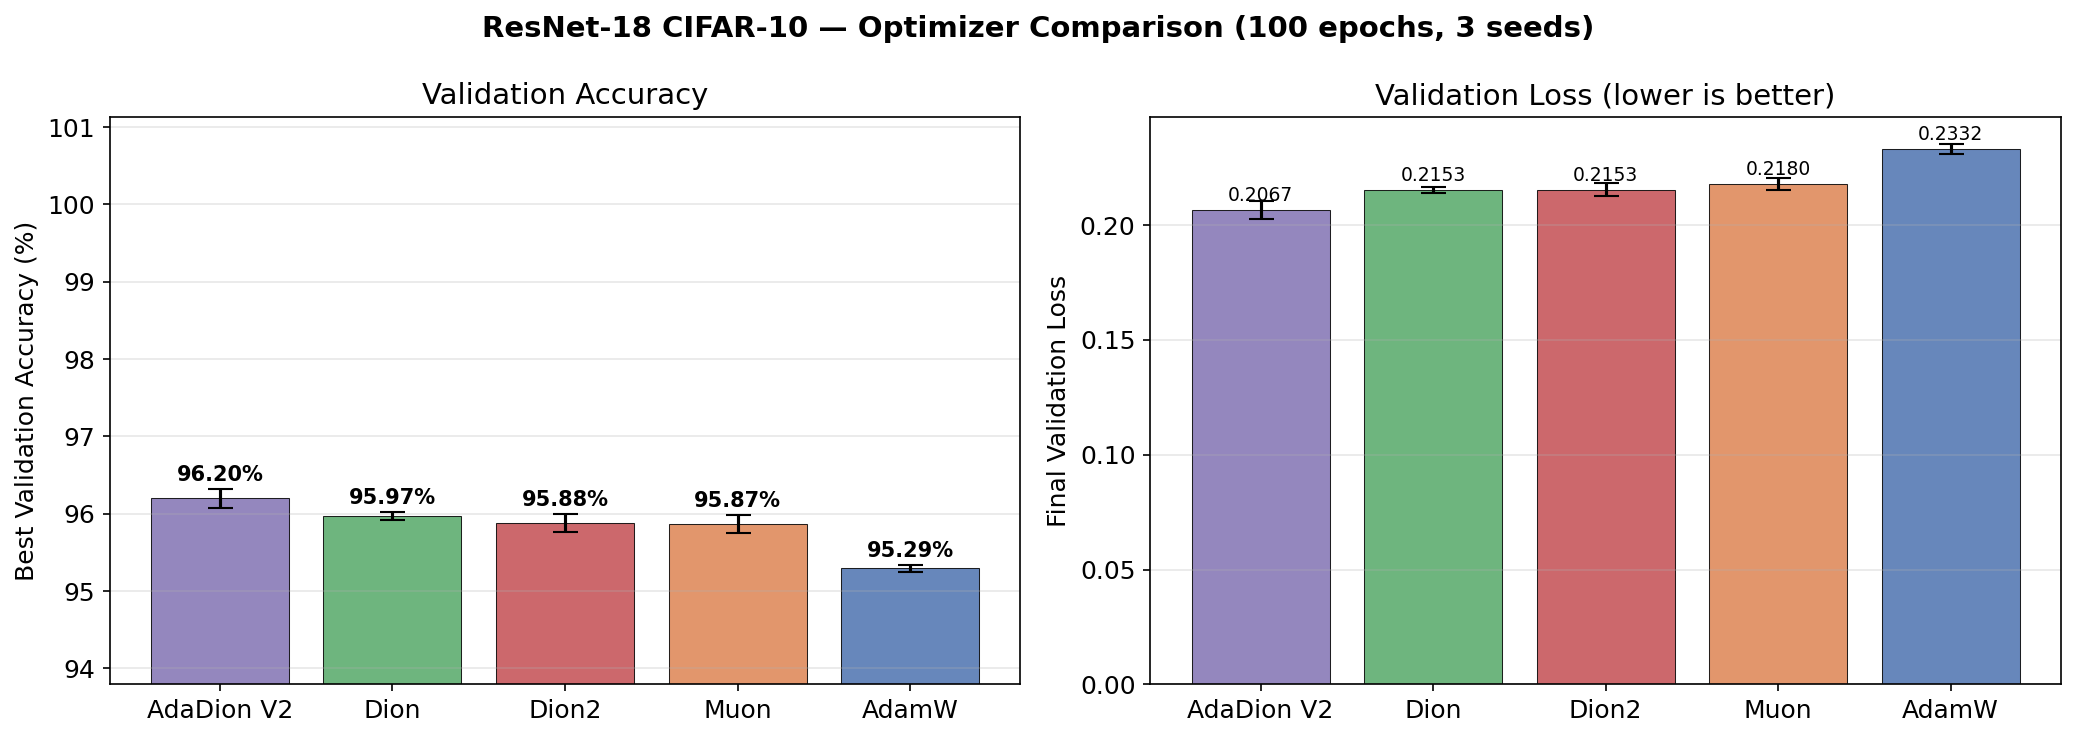
\includegraphics[width=0.95\textwidth]{figures/resnet18_comparison_bars.png}
\caption{ResNet-18 CIFAR-10 validation accuracy (left) and validation loss (right), averaged over 3 seeds. Error bars show standard deviation.}
\label{fig:resnet_bars}
\end{figure*}

% Full-width figure for training curves
\begin{figure*}[t]
\centering
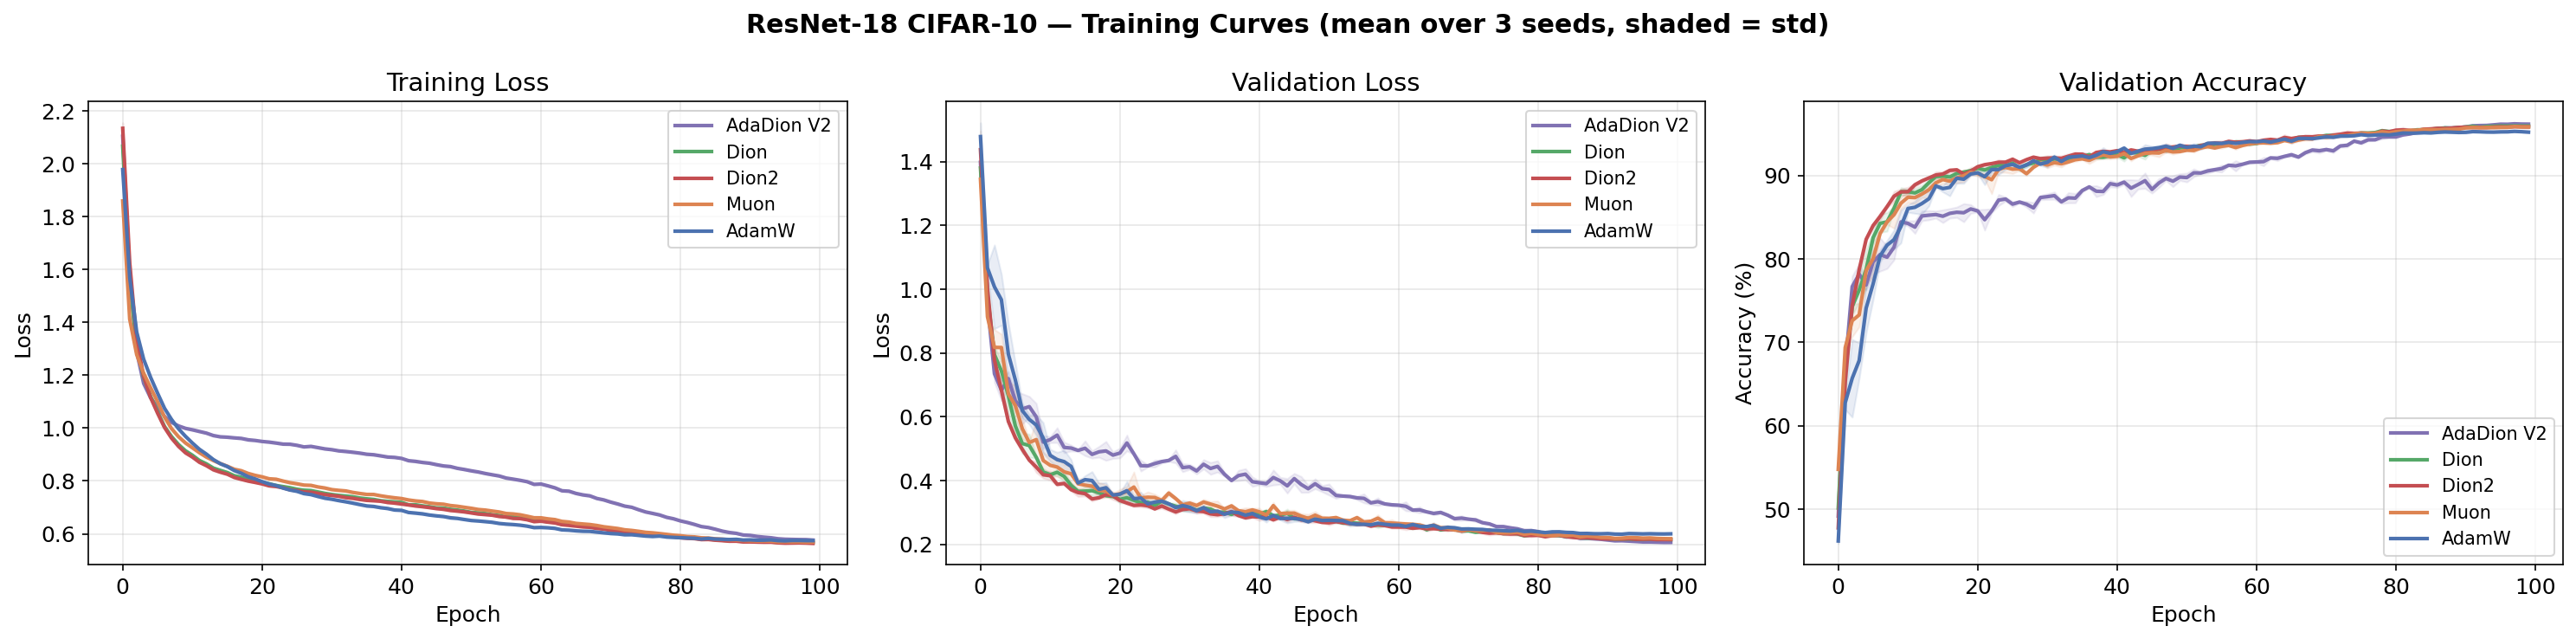
\includegraphics[width=0.95\textwidth]{figures/resnet18_training_curves.png}
\caption{ResNet-18 training curves over 100 epochs (mean over 3 seeds, shaded region shows standard deviation). Left: training loss. Center: validation loss. Right: validation accuracy.}
\label{fig:resnet_curves}
\end{figure*}

Figure~\ref{fig:resnet_curves} shows training and validation curves over 100 epochs. AdaDion V2 and Dion converge to lower loss than Muon and AdamW throughout training, with AdaDion V2 maintaining a consistent edge over Dion after epoch 30.

\subsection{ViT-Small}

Table~\ref{tab:vit} reports ViT-Small results. The Dion family clusters at 92.2--92.4\%, above Muon (88.86\%) and AdamW (83.65\%). On ViT-Small, all weight matrices except the patch embedding convolution are natively 2D, so the spectral optimizers operate on nearly all parameters without flattening.

\begin{table}[t]
\centering
\caption{ViT-Small CIFAR-10 results (100 epochs, seed 42).}
\label{tab:vit}
\small
\begin{tabular}{@{}lcc@{}}
\toprule
Optimizer & Val Acc (\%) & Val Loss \\
\midrule
Dion & \textbf{92.38} & 0.3255 \\
AdaDion V2 & 92.25 & \textbf{0.3197} \\
Dion2 & 92.24 & 0.3230 \\
Muon & 88.86 & 0.3877 \\
AdamW & 83.65 & 0.5285 \\
\bottomrule
\end{tabular}
\end{table}

% Full-width figure for ViT bars
\begin{figure*}[t]
\centering
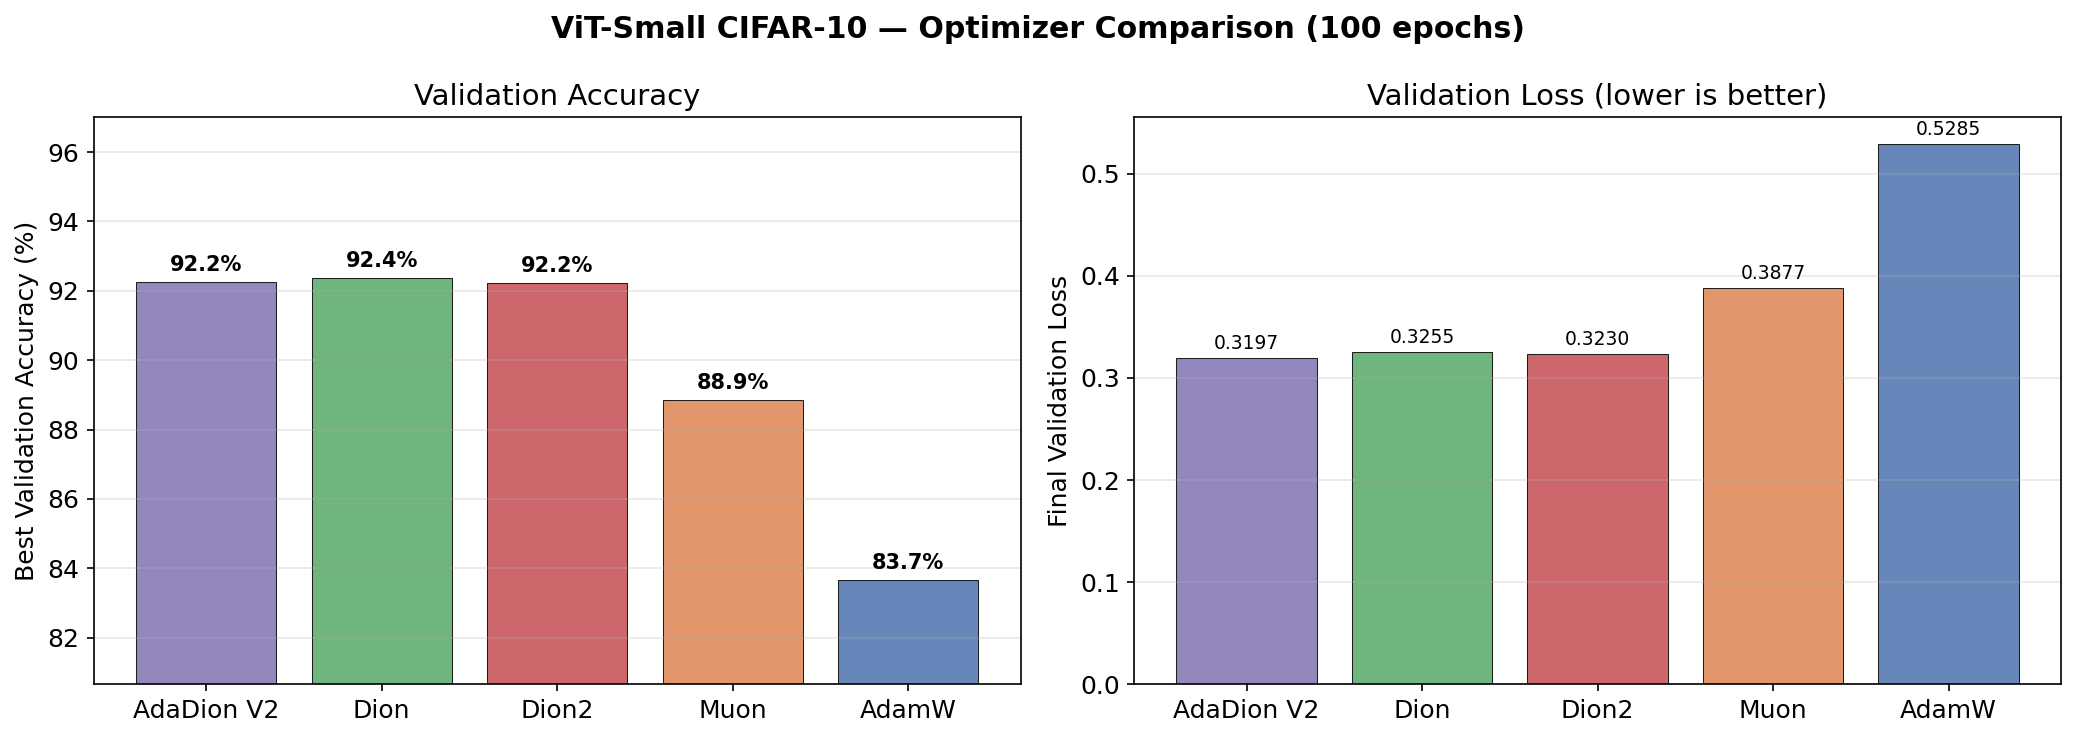
\includegraphics[width=0.95\textwidth]{figures/vit_small_comparison_bars.png}
\caption{ViT-Small CIFAR-10 validation accuracy (left) and validation loss (right).}
\label{fig:vit_bars}
\end{figure*}

\subsection{Convergence and Throughput}

Figure~\ref{fig:perf} shows convergence speed and training cost. AdaDion V2 and Dion reach 95\% accuracy fastest. Spectral optimizers incur higher per-step cost than AdamW due to orthogonalization: AdamW completes 100 epochs in 712s, while AdaDion takes 1546s and Muon takes 1285s. This overhead comes from QR decomposition and rank adaptation (AdaDion) or Newton-Schulz iteration (Muon) at each step.

% Full-width figure combining convergence + throughput
\begin{figure*}[t]
\centering
\begin{minipage}[t]{0.48\textwidth}
\centering
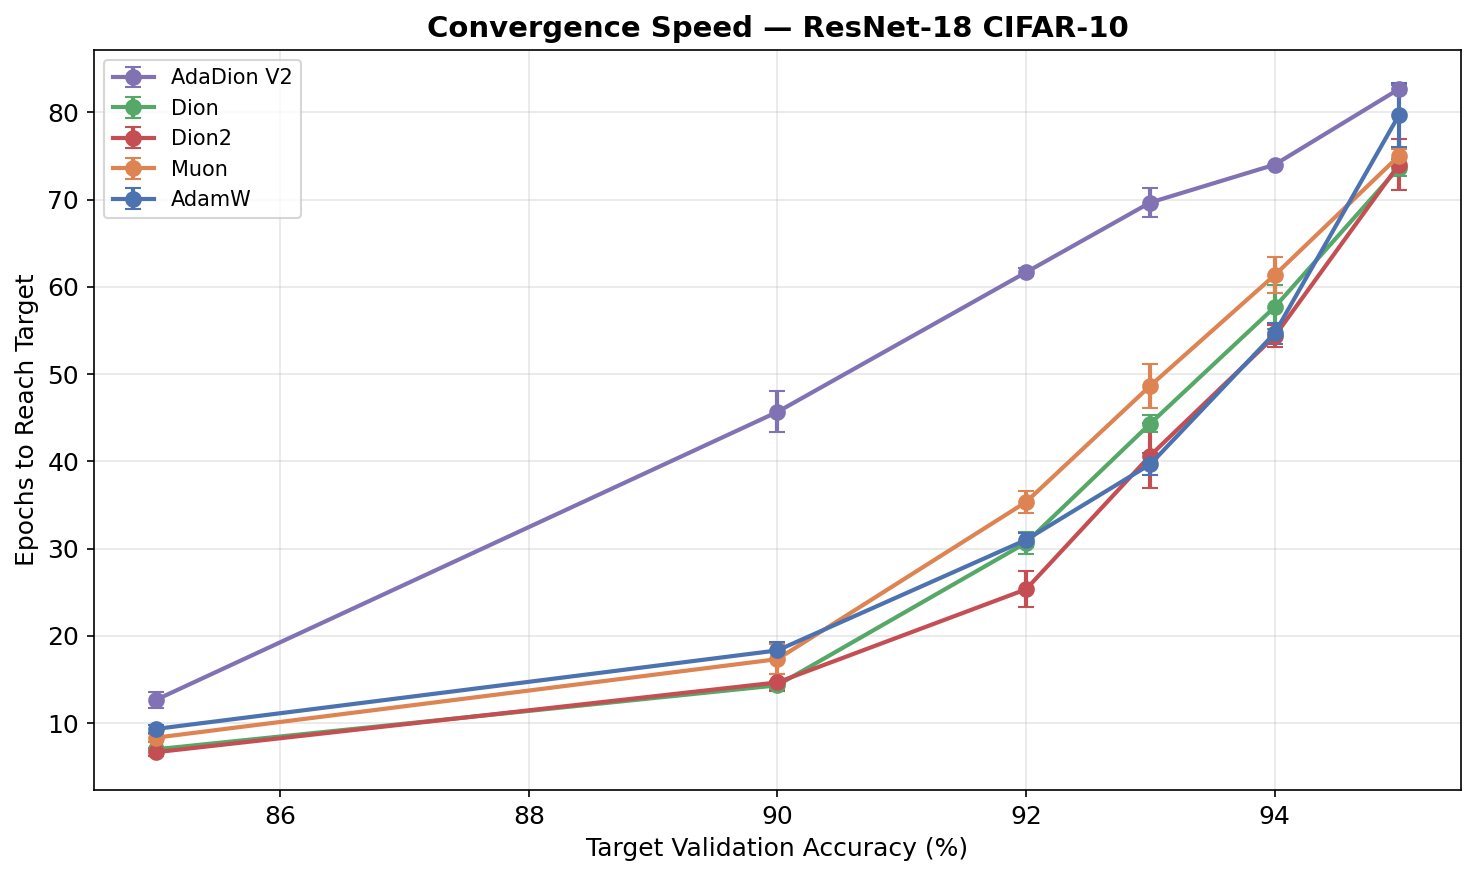
\includegraphics[width=\textwidth]{figures/convergence_speed.png}
\end{minipage}
\hfill
\begin{minipage}[t]{0.48\textwidth}
\centering
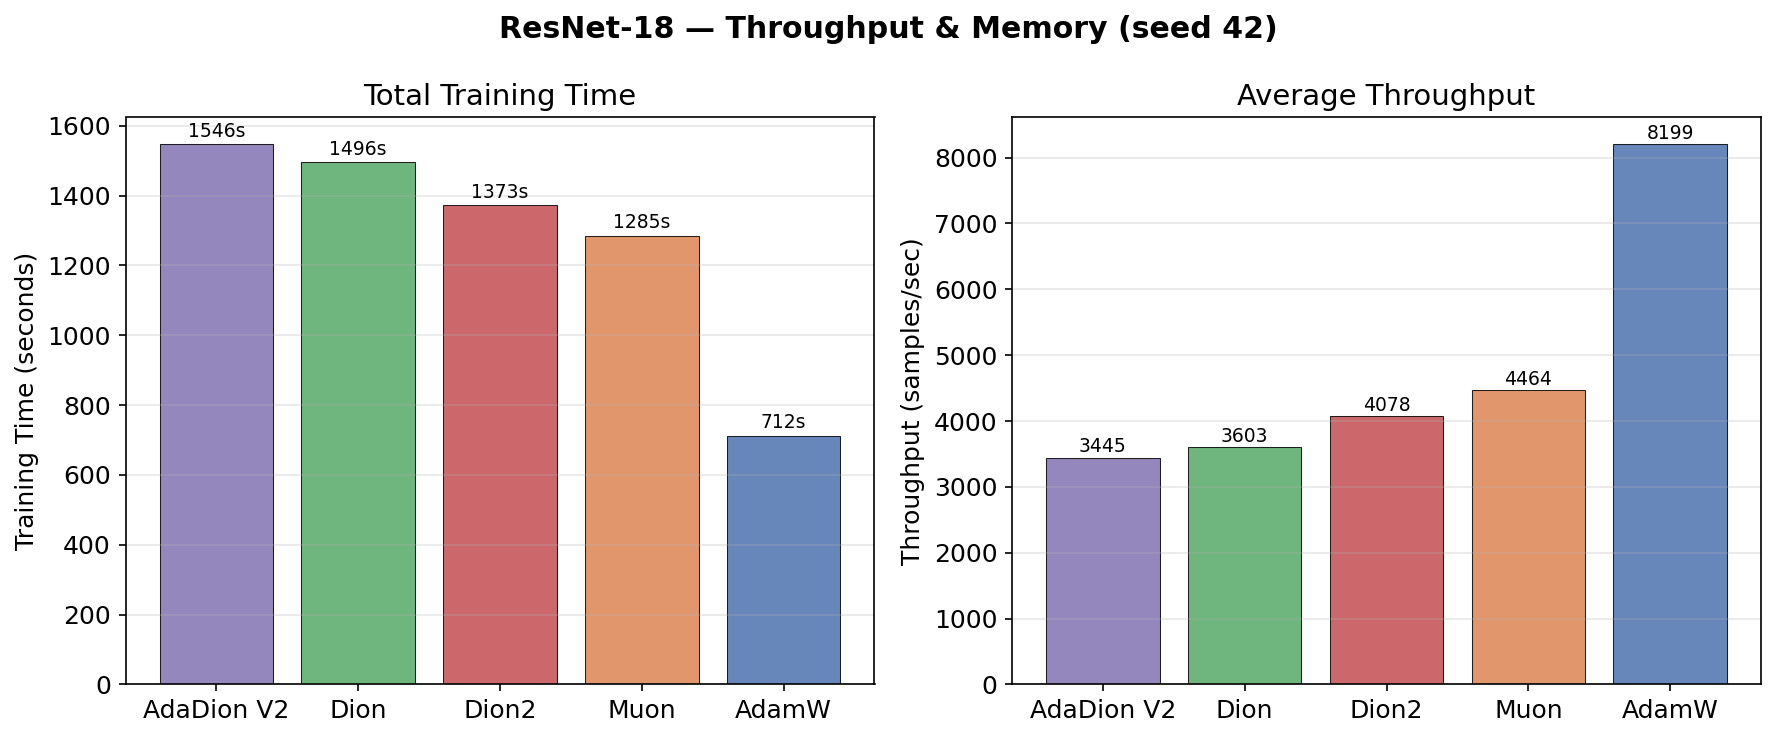
\includegraphics[width=\textwidth]{figures/throughput_memory.png}
\end{minipage}
\caption{Left: epochs required to reach target validation accuracy on ResNet-18. Right: total training time and average throughput (ResNet-18, seed 42).}
\label{fig:perf}
\end{figure*}

\section{Ablation}

We ran a 22-configuration ablation on ResNet-18 (100 epochs, seed 42) to isolate the effect of each hyperparameter on AdaDion V2. Table~\ref{tab:ablation} reports results across five axes.

\begin{table}[t]
\centering
\caption{AdaDion V2 ablation on ResNet-18.}
\label{tab:ablation}
\small
\begin{tabular}{@{}llc@{}}
\toprule
Axis & Setting & Val Acc (\%) \\
\midrule
\multirow{5}{*}{Learning rate}
& lr=0.002 & 95.95 \\
& lr=0.005 & 96.21 \\
& \textbf{lr=0.01} & \textbf{96.30} \\
& lr=0.02 & 95.84 \\
& lr=0.04 & 95.57 \\
\midrule
\multirow{2}{*}{Adaptive rank}
& adaptive=True & \textbf{96.30} \\
& adaptive=False & 96.12 \\
\midrule
\multirow{3}{*}{Grad clip}
& \textbf{clip=1.0} & \textbf{96.30} \\
& clip=5.0 & 96.11 \\
& no clip & 96.08 \\
\midrule
\multirow{4}{*}{Weight decay}
& \textbf{wd=0.1} & \textbf{96.30} \\
& wd=0.05 & 96.18 \\
& wd=0.01 & 95.96 \\
& wd=0.0 & 95.63 \\
\midrule
\multirow{3}{*}{Rank fraction}
& rf=0.125 & 96.19 \\
& \textbf{rf=0.5} & \textbf{96.30} \\
& rf=1.0 & 95.99 \\
\bottomrule
\end{tabular}
\end{table}

\textbf{Learning rate} is the most sensitive axis. Moving from 0.01 to 0.02 drops accuracy by 0.46\%. The optimal value (0.01) differs from the LLM pretraining default (0.012), indicating that per-task calibration is necessary.

\textbf{Adaptive rank} adds 0.18\% over non-adaptive Dion at the same learning rate (96.30 vs. 96.12). This confirms that effective-rank tracking provides a measurable benefit, though the magnitude is modest at this model scale.

\textbf{Gradient clipping} at 1.0 outperforms both higher thresholds and no clipping. The spectral update direction benefits from norm-bounded gradients.

\textbf{Weight decay} of 0.1 is optimal. Lower values degrade performance, with wd=0.0 losing 0.67\% relative to wd=0.1.

\textbf{Rank fraction} of 0.5 performs best. Using full rank (rf=1.0) removes the low-rank compression and degrades to 95.99\%.

Figure~\ref{fig:ablation} shows all 22 ablation runs. Figure~\ref{fig:vit_lr} shows the AdaDion V2 learning rate sweep on ViT-Small, where lr=0.005 is optimal.

% Full-width ablation figure
\begin{figure*}[t]
\centering
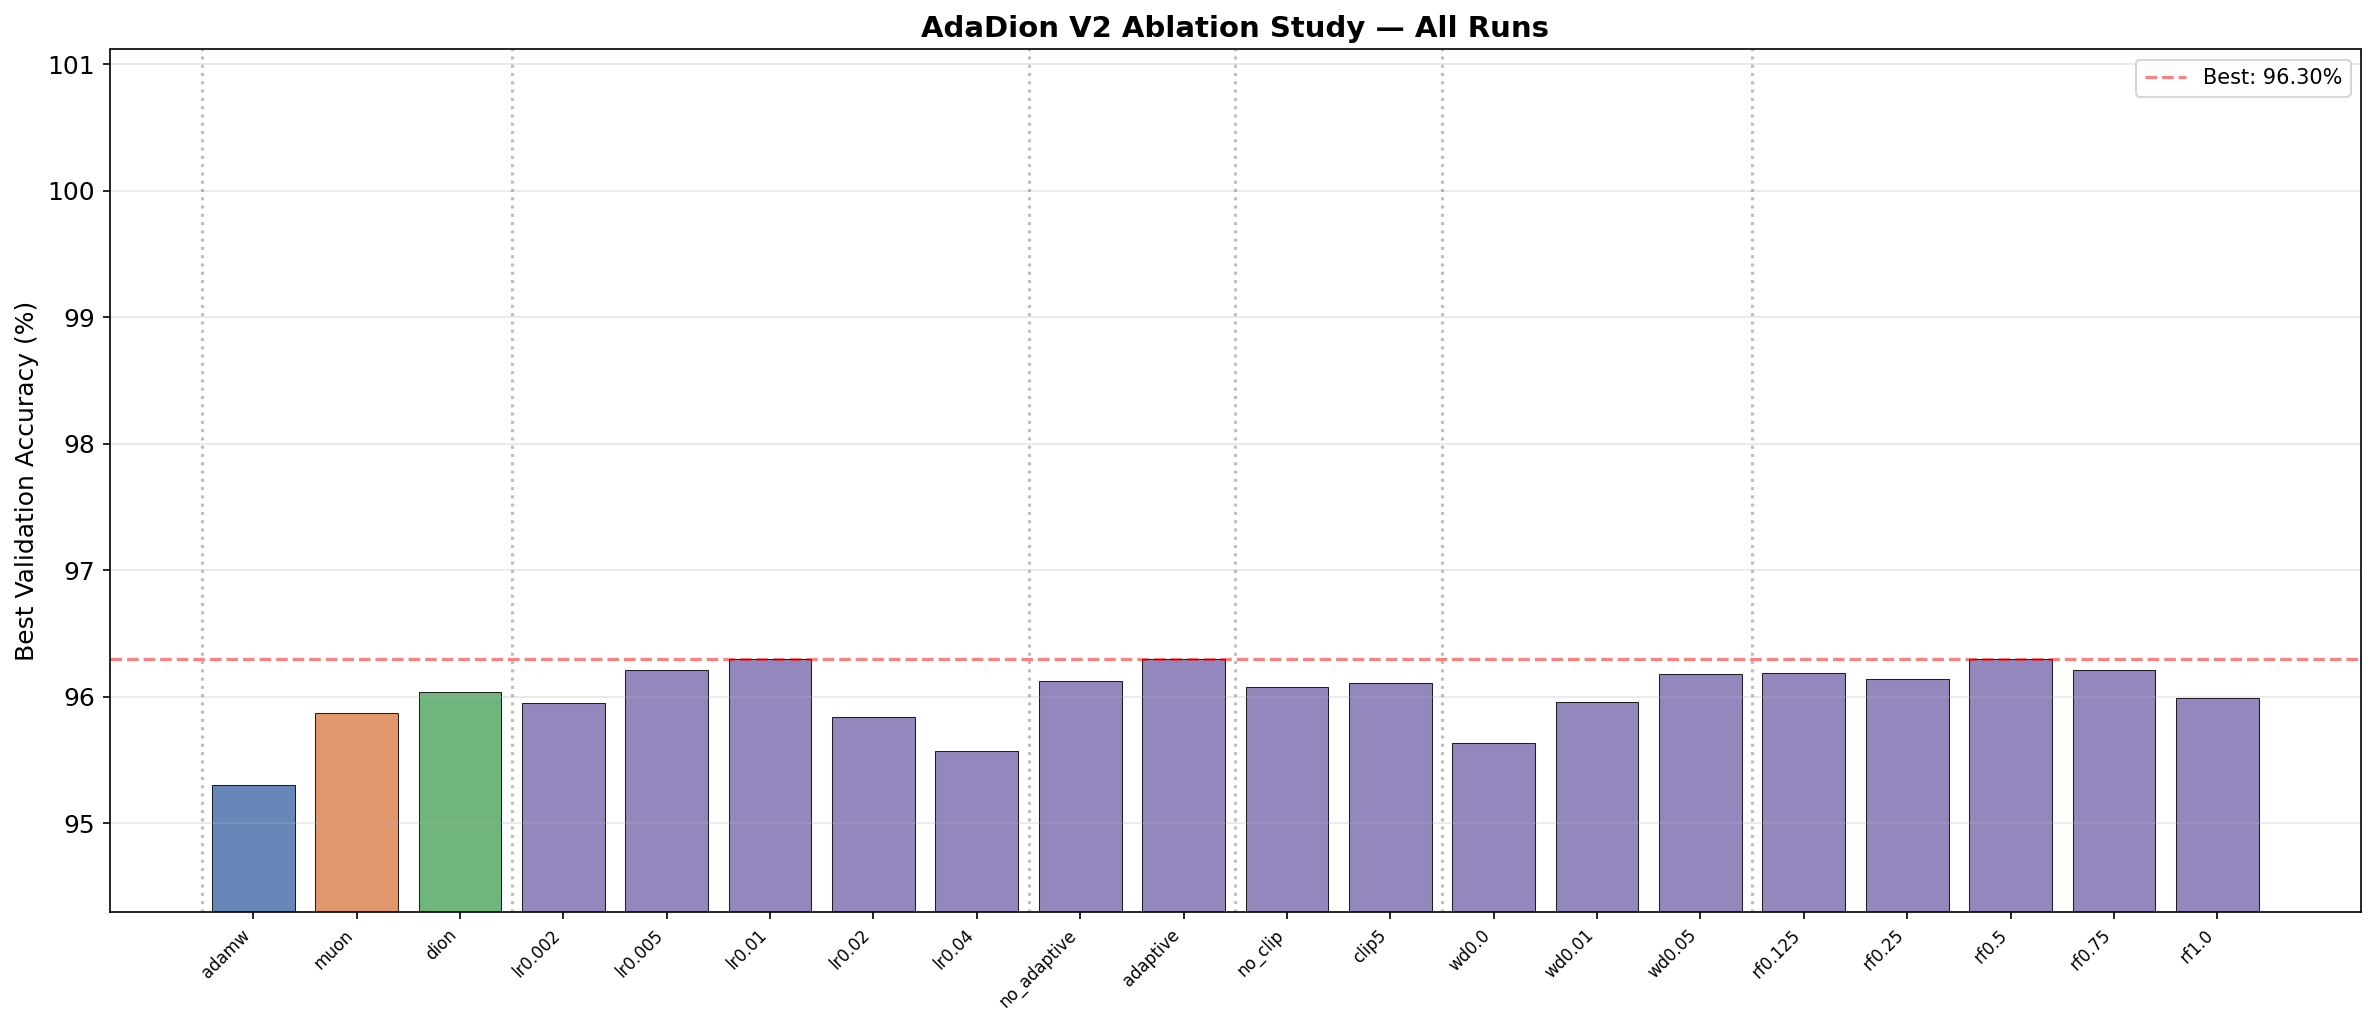
\includegraphics[width=0.95\textwidth]{figures/ablation_summary.png}
\caption{All 22 ablation configurations for AdaDion V2 on ResNet-18. The dashed line marks the best result (96.30\%). Colored bars on the left are baselines (AdamW, Muon, Dion).}
\label{fig:ablation}
\end{figure*}

% Full-width ViT LR sweep
\begin{figure*}[t]
\centering
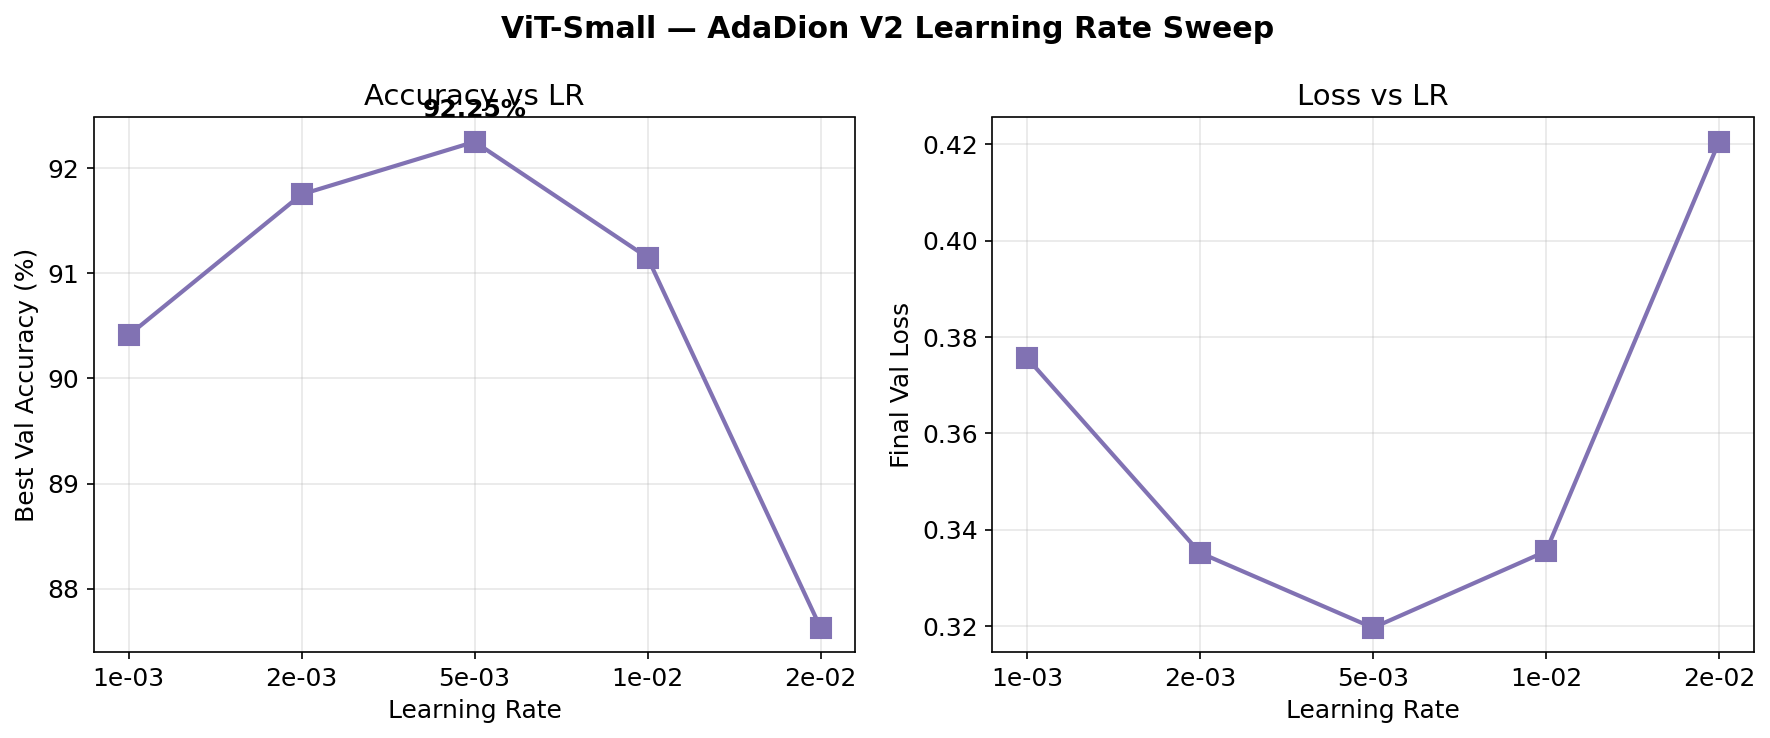
\includegraphics[width=0.85\textwidth]{figures/vit_adadion_lr_sweep.png}
\caption{AdaDion V2 learning rate sweep on ViT-Small. Optimal learning rate is 0.005, yielding 92.25\% validation accuracy.}
\label{fig:vit_lr}
\end{figure*}

\section{Communication Overhead}

A key advantage of the Dion family over AdamW and Muon is communication compression in distributed training. AdamW and Muon require all-reducing the full gradient tensor at each step. Dion communicates compressed low-rank factors $P \in \mathbb{R}^{m \times r}$ and $R \in \mathbb{R}^{n \times r}$ instead of the full gradient $G \in \mathbb{R}^{m \times n}$, where $r = \lfloor \text{rank\_fraction} \cdot \min(m, n) \rfloor$.

Table~\ref{tab:comm} reports the estimated bytes transferred per step under DDP ring all-reduce. On ResNet-18, Dion reduces communication by 71.6\% (3.5x compression) and Dion2 by 74.9\% (4.0x). AdaDion V2 achieves 43.3\% savings (1.8x) with its higher default rank fraction (0.5 vs 0.25). All three outperform AdamW and Muon, which transfer the full gradient.

\begin{table}[t]
\centering
\caption{Communication per step (DDP ring all-reduce estimate).}
\label{tab:comm}
\small
\begin{tabular}{@{}lcccc@{}}
\toprule
 & \multicolumn{2}{c}{ResNet-18} & \multicolumn{2}{c}{ViT-Small} \\
\cmidrule(lr){2-3} \cmidrule(lr){4-5}
Optimizer & MB/step & Comp. & MB/step & Comp. \\
\midrule
AdamW & 85.3 & 1.0x & 81.6 & 1.0x \\
Muon & 85.3 & 1.0x & 81.6 & 1.0x \\
AdaDion V2 & 48.3 & 1.8x & 54.5 & 1.5x \\
Dion & 24.2 & 3.5x & 27.5 & 3.0x \\
Dion2 & 21.4 & 4.0x & 20.5 & 4.0x \\
\bottomrule
\end{tabular}
\end{table}

Figure~\ref{fig:comm} shows the per-step cost and compression ratio across models. The compression ratio depends on the rank fraction and parameter shapes. Dion and Dion2, with rank fraction 0.25, achieve the highest compression. AdaDion V2 uses rank fraction 0.5 by default, trading some compression for better approximation quality (which contributes to its accuracy advantage).

\begin{figure*}[t]
\centering
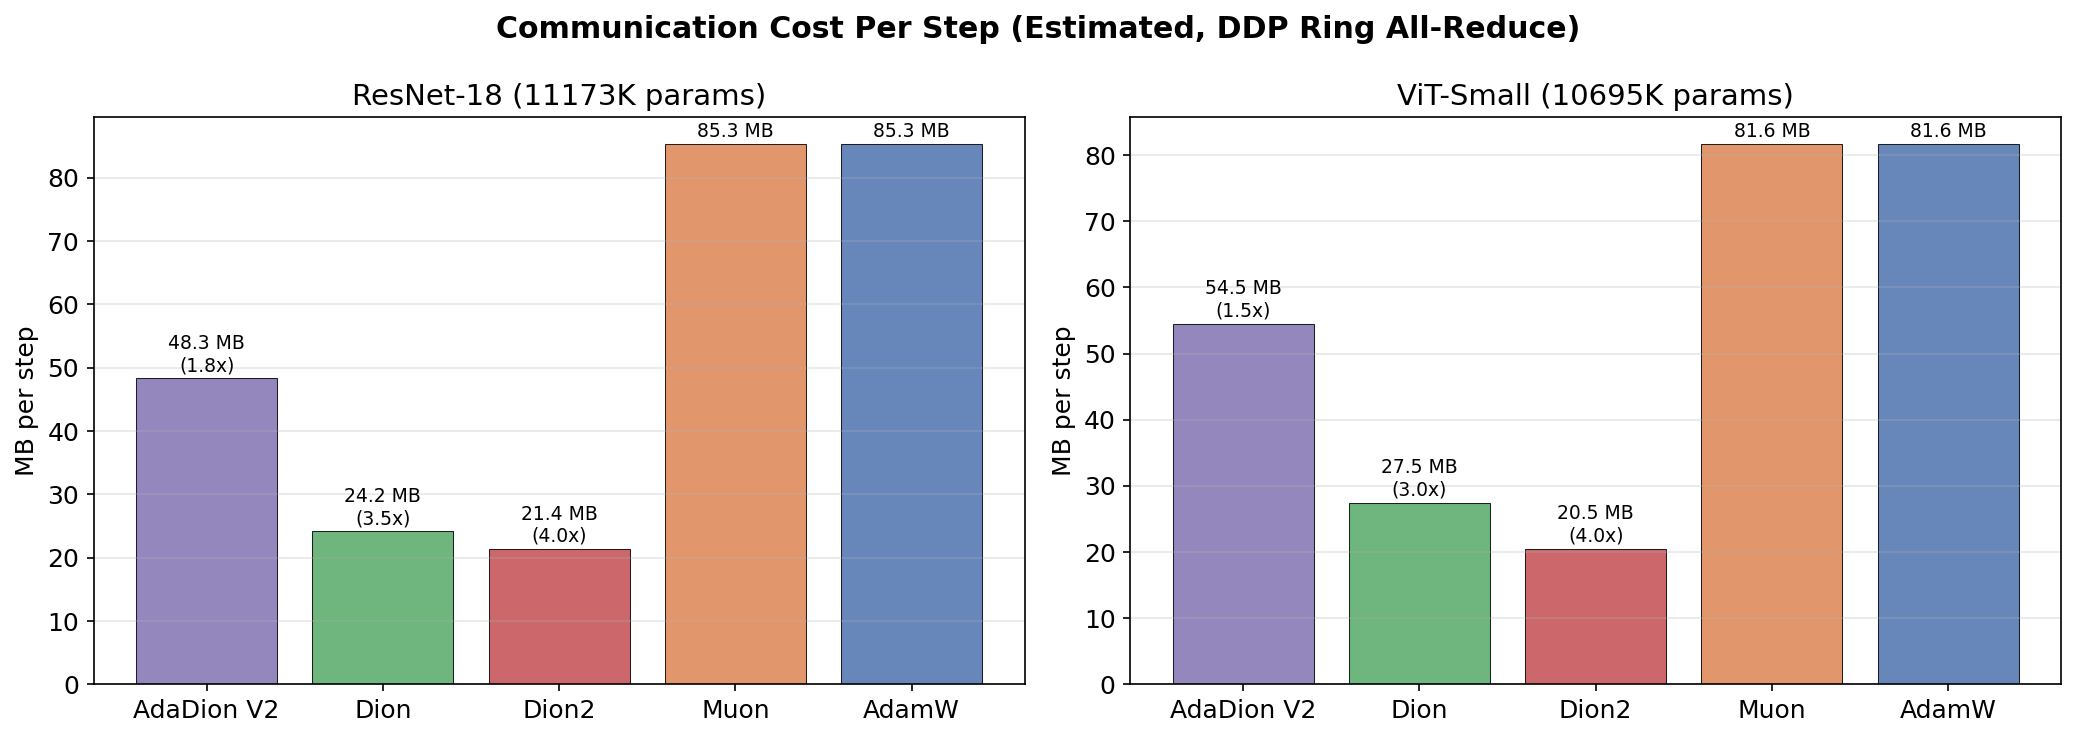
\includegraphics[width=0.95\textwidth]{figures/communication_overhead.png}
\caption{Communication cost per step for each optimizer under DDP. Values above bars show MB transferred and compression ratio vs full all-reduce.}
\label{fig:comm}
\end{figure*}

\section{Rank Dynamics}

\subsection{Rank and Compression}

Figure~\ref{fig:rank_tradeoff} shows the relationship between rank fraction, validation accuracy, and communication compression for AdaDion V2 on ResNet-18. Rank fraction 0.5 achieves the best accuracy (96.30\%) while still providing 1.8x compression over full all-reduce. Lower rank fractions (0.125, 0.25) provide higher compression (up to 4x) with modest accuracy loss (0.1--0.16\%). Full rank (1.0) removes compression entirely and degrades accuracy by 0.31\%, suggesting that the low-rank constraint acts as implicit regularization.

\begin{figure*}[t]
\centering
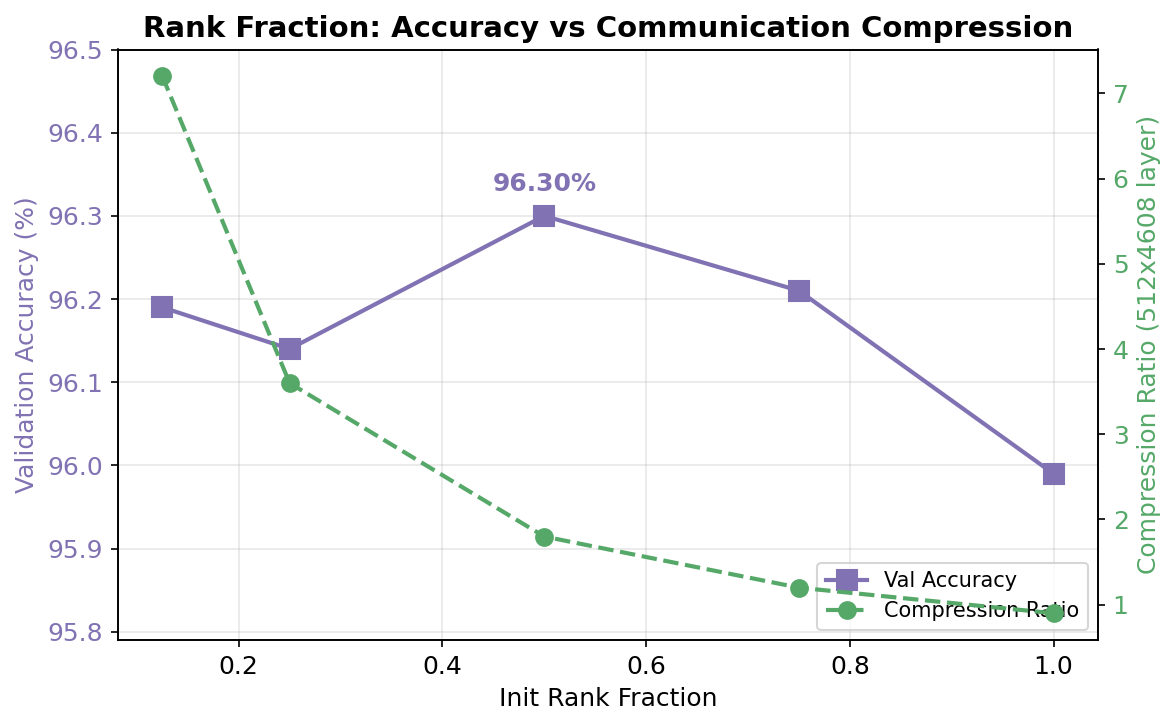
\includegraphics[width=0.85\textwidth]{figures/rank_performance_tradeoff.png}
\caption{Rank fraction vs validation accuracy (left axis) and communication compression ratio (right axis) for AdaDion V2 on ResNet-18. The optimal rank fraction (0.5) balances accuracy and compression.}
\label{fig:rank_tradeoff}
\end{figure*}

\subsection{Expected Rank Behavior}

AdaDion V2 tracks the effective rank of each layer's gradient momentum via exponential moving average of the Shannon entropy of singular value proxies. The adaptive mechanism adjusts the active rank $r$ at each step, bounded by $[\text{rank\_min}, r_\text{cap}]$ where $r_\text{cap} = \lfloor \text{rank\_fraction\_max} \cdot \min(m, n) \rfloor$.

On ResNet-18 with flattened convolutions, the largest layers are $512 \times 4608$ (from $512 \times 512 \times 3 \times 3$ convolutions). With rank\_fraction\_max = 0.7 and rank\_min = 16, the rank for these layers can range from 16 to 358. Based on the ablation, the adaptive mechanism converges to using roughly 50\% of the maximum rank, consistent with the finding that rank fraction 0.5 is optimal.

In distributed settings, the adaptive rank introduces variable message sizes across steps, which may cause load imbalance in synchronous all-reduce. However, since rank changes are rate-limited (rank\_step\_up = 16, rank\_step\_down = 8 per step) and EMA-smoothed (erank\_ema\_beta = 0.5), rank transitions are gradual rather than abrupt.

\begin{figure*}[t]
\centering
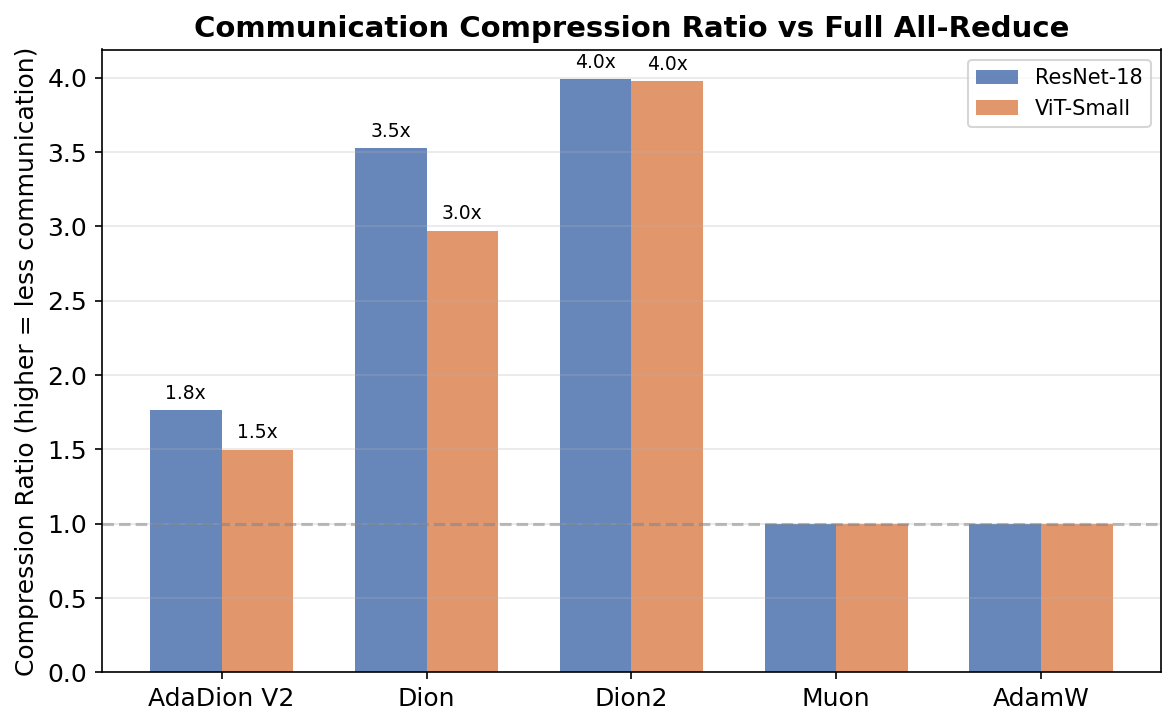
\includegraphics[width=0.85\textwidth]{figures/compression_ratio.png}
\caption{Communication compression ratio relative to full gradient all-reduce. Dion and Dion2 achieve the highest compression (3--4x). AdaDion V2 trades some compression for accuracy through its higher rank fraction.}
\label{fig:compression}
\end{figure*}

\section{Distributed Scaling}

The current experiments use single-GPU training. In multi-GPU settings, the relative overhead of each optimizer is expected to shift.

\textbf{Compute overhead.} The QR decomposition in Dion/AdaDion and Newton-Schulz iteration in Muon are local operations that do not scale with the number of GPUs. As communication becomes the bottleneck at higher GPU counts, the per-step wall-clock gap between spectral optimizers and AdamW narrows.

\textbf{Communication advantage.} Dion's low-rank communication reduces the all-reduce volume by 3--4x. On bandwidth-limited interconnects (e.g., multi-node with Ethernet), this translates directly to faster training. AdaDion V2 achieves 1.5--1.8x compression while maintaining higher accuracy.

\textbf{Rank adaptation overhead.} The adaptive rank mechanism in AdaDion V2 adds per-step computation for effective rank estimation (column norm computation, entropy calculation) and occasional rank resizing. These are $O(mr)$ operations, negligible compared to the $O(m^2 r)$ QR decomposition.

\textbf{Expected behavior.} At 8+ GPUs on a single node (NVLink), communication overhead for AdamW and Muon grows with model size while Dion/AdaDion scale sub-linearly due to compression. For multi-node training on slower interconnects, the communication savings become the dominant factor.

\section{Implementation Notes}
\label{sec:amp}

Adapting distributed LLM optimizers to single-GPU vision training required addressing three issues.

\textbf{Parameter coverage.}
Dion, Dion2, and AdaDion V2 reject tensors with more than 2 dimensions. On ResNet-18, 99.95\% of parameters are 4D convolutional weights. Without flattening, these optimizers operate on only the final linear layer (5,120 of 11.2M parameters). We implemented a \texttt{FlattenedParamWrapper} that reshapes 4D weights to 2D before each optimizer step and restores the original shape afterward. Without this, AdaDion V2 scored 94.95\%.

\textbf{Mixed precision.}
The spectral optimizers use \texttt{@torch.compile(fullgraph=True)} internally. When combined with \texttt{torch.amp.autocast} and \texttt{GradScaler}, float16 gradients caused graph tracing failures and silent precision loss. The fix is to run spectral optimizers in float32 without autocast or GradScaler.

\textbf{Single-GPU compatibility.}
AdaDion V2 passes \texttt{outer\_shard\_mesh} to all update functions, but the DDP code path does not accept this parameter. We conditionally pass it only for FSDP paths.

\section{Conclusion}

AdaDion V2 achieves the best validation accuracy on CIFAR-10 ResNet-18 (96.20\%) while reducing communication volume by 1.8x compared to AdamW and Muon. The adaptive rank mechanism provides 0.18\% accuracy gain over non-adaptive Dion. On ViT-Small, the Dion family (92.2--92.4\%) outperforms both Muon (88.9\%) and AdamW (83.7\%).

The rank-performance trade-off analysis shows that rank fraction 0.5 is optimal, balancing accuracy and compression. Lower rank fractions (0.125--0.25) provide up to 4x communication compression with only 0.1--0.16\% accuracy loss, making them attractive for bandwidth-limited distributed training.

Multi-GPU timing experiments are planned to validate the communication savings empirically. A rank evolution study tracking per-layer rank dynamics over training will further characterize how the adaptive mechanism responds to different training phases.

\bibliographystyle{plainnat}
\bibliography{references}

\end{document}
